\documentclass[aspectratio=169]{beamer}

% -------------------------
% Packages
% -------------------------
\usepackage[utf8]{inputenc}
\usepackage{graphicx}
\usepackage{amsmath, amssymb}
\usepackage{booktabs}
\usepackage{tcolorbox}
\usepackage{tikz}
\definecolor{questionbg}{RGB}{235, 244, 255}
\definecolor{questionframe}{RGB}{44, 95, 173}
\definecolor{plainbg}{RGB}{241, 249, 241}
\definecolor{plainframe}{RGB}{44, 122, 70}
\definecolor{notationbg}{RGB}{255, 248, 230}
\definecolor{notationframe}{RGB}{176, 118, 0}

\newtcolorbox{questionbox}{
  colback=questionbg,
  colframe=questionframe,
  boxrule=0.7pt,
  arc=1mm,
  fontupper=\small,
  left=1mm,
  right=1mm,
  top=0.4mm,
  bottom=0.4mm
}

\newtcolorbox{plainbox}{
  colback=plainbg,
  colframe=plainframe,
  boxrule=0.7pt,
  arc=1mm,
  fontupper=\small,
  left=1mm,
  right=1mm,
  top=0.4mm,
  bottom=0.4mm
}

\newtcolorbox{notationbox}{
  colback=notationbg,
  colframe=notationframe,
  boxrule=0.7pt,
  arc=1mm,
  fontupper=\small,
  left=1mm,
  right=1mm,
  top=0.4mm,
  bottom=0.4mm
}

\newcommand{\keyquestion}[1]{%
  \begin{questionbox}
  \textbf{Question:} #1
  \end{questionbox}
}

\newcommand{\plainidea}[1]{%
  \begin{plainbox}
  \textbf{Main idea:} #1
  \end{plainbox}
}

\newcommand{\notationblock}[1]{%
  \begin{notationbox}
  \textbf{Symbols used on this slide}\\
  #1
  \end{notationbox}
}

\newcommand{\exercisebreakcontent}[1]{%
  \begin{center}
  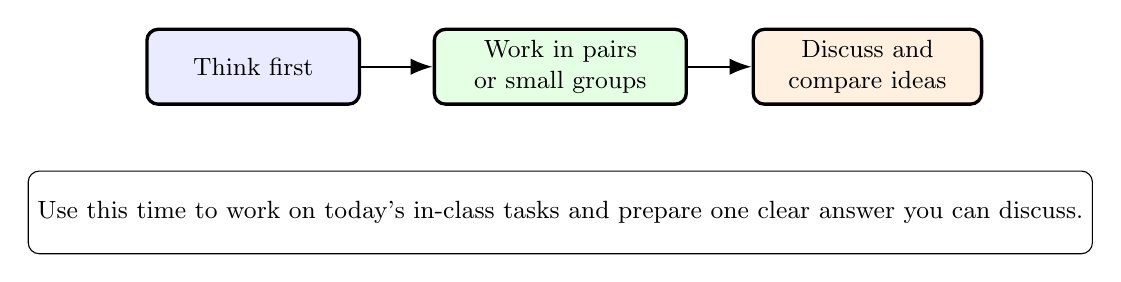
\begin{tikzpicture}[>=Latex, every node/.style={font=\small}]
    \node[draw, rounded corners, very thick, fill=blue!8, minimum width=2.7cm, minimum height=0.95cm, align=center] (think) at (-3.9,0.9) {Think first};
    \node[draw, rounded corners, very thick, fill=green!10, minimum width=3.2cm, minimum height=0.95cm, align=center] (work) at (0,0.9) {Work in pairs\\or small groups};
    \node[draw, rounded corners, very thick, fill=orange!12, minimum width=2.9cm, minimum height=0.95cm, align=center] (share) at (3.9,0.9) {Discuss and\\compare ideas};
    \draw[-{Latex[length=2.8mm]}, thick] (think) -- (work);
    \draw[-{Latex[length=2.8mm]}, thick] (work) -- (share);
    \node[draw, rounded corners, fill=white, minimum width=9.4cm, minimum height=1.05cm, align=center] at (0,-0.95) {Use this time to work on today's in-class tasks and prepare one clear answer you can discuss.};
  \end{tikzpicture}
  \end{center}
  \plainidea{#1}
}

\usepackage{hyperref}
\usetikzlibrary{positioning,arrows.meta,shapes.geometric}

% -------------------------
% Theme
% -------------------------
\usetheme{Madrid}
\usecolortheme{default}
\setbeamertemplate{navigation symbols}{}

% -------------------------
% Per-slide reference footer
% -------------------------
\newcommand{\defaultdeckrefs}{AIMA4e Ch.10 pp.314--343; Poole3e Ch.16 pp.701--730}
\newcommand{\currentsliderefs}{\defaultdeckrefs}
\newcommand{\setslideref}[1]{\gdef\currentsliderefs{#1}}
\addtobeamertemplate{footline}{}{%
  \begin{beamercolorbox}[wd=\paperwidth,leftskip=0.4em,rightskip=0.4em,ht=2.8ex,dp=0.9ex]{author in head/foot}
    \tiny\textbf{Refs: }\currentsliderefs
  \end{beamercolorbox}
}

% -------------------------
% Metadata
% -------------------------
\title[EBU6505 Block 3 Day 2]{EBU6505 -- Reasoning and Agents\\Block 3, Day 2 -- Knowledge Representation}
\author{Dr Riasat Islam}
\institute{Queen Mary University of London}
\date{}

\begin{document}

% 1
\setslideref{AIMA4e Ch.10 pp.314--343; Poole3e Ch.16 pp.701--730}
\begin{frame}
  \titlepage
\end{frame}

% 2
\setslideref{AIMA4e Ch.10 pp.314--343; Poole3e Ch.16 pp.701--730}
\begin{frame}{What have we covered so far this week?}
\begin{itemize}
  \item Sequential decision making and MDP components
  \item Return, discounting, value, and Bellman intuition
  \item Why reward and state matter in sequential decision problems
\end{itemize}
\plainidea{Yesterday introduced sequential decision models and reward over time. Today is about storing facts in a form an agent can search and reason over.}
\end{frame}

% 3
\setslideref{AIMA4e Ch.10 pp.314--343; Poole3e Ch.16 pp.701--730}
\begin{frame}{What are we going to cover today?}
\begin{itemize}
  \item Why AI systems need explicit knowledge representation
  \item Entities, relations, attributes, triples, and identifiers
  \item Schema graphs versus instance graphs
  \item Why structured knowledge helps search, retrieval, and agent memory
\end{itemize}
\plainidea{The goal of today is simple: take a normal sentence and turn it into a machine-usable structure.}
\end{frame}

% 4
\setslideref{AIMA4e Ch.10 pp.314--343; Poole3e Ch.16 pp.701--730}
\begin{frame}{Resources}
\begin{itemize}
  \item \textit{Artificial Intelligence: Foundations of Computational Agents}, David Poole and Alan Mackworth (3rd ed.)
  \item Chapter 16 -- knowledge graphs, graph modelling, and structured knowledge
  \item \textit{Artificial Intelligence: A Modern Approach}, Russell and Norvig (4th ed.)
  \item Chapter 10 -- knowledge representation
\end{itemize}
\plainidea{Read the textbooks for the formal view. In class, we focus on the intuition and the patterns used in modern AI systems.}
\end{frame}

% 5
\setslideref{AIMA4e Ch.10 pp.314--343; Poole3e Ch.16 pp.701--730}
\begin{frame}{Learning Outcomes for Today}
By the end of this session, you should be able to:
\begin{itemize}
  \item explain why plain text alone is often not enough for reasoning systems
  \item represent simple facts as triples
  \item distinguish entities, relations, attributes, and identifiers
  \item explain how search systems and modern agents use structured knowledge
\end{itemize}
\end{frame}

% 6
\setslideref{AIMA4e Ch.10 pp.314--343; Poole3e Ch.16 pp.701--730}
\begin{frame}{Warm-up Exercise}
\keyquestion{Can you write one real-world fact so that a machine could store it clearly?}
\begin{columns}[T,onlytextwidth]
  \begin{column}{0.48\textwidth}
    \begin{itemize}
      \item Try one short example before the lecture continues.
      \item Write the fact in a way that removes ambiguity.
    \end{itemize}
  \end{column}
  \begin{column}{0.48\textwidth}
    \begin{center}
    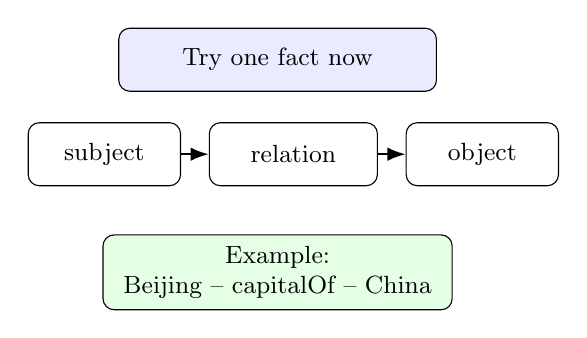
\begin{tikzpicture}[>=Latex, every node/.style={font=\small}]
      \node[draw, rounded corners, fill=blue!8, text width=3.8cm, minimum height=0.8cm, align=center] at (0,1.2) {Try one fact now};
      \node[draw, rounded corners, fill=white, text width=1.7cm, minimum height=0.8cm, align=center] (s) at (-2.2,0) {subject};
      \node[draw, rounded corners, fill=white, text width=1.9cm, minimum height=0.8cm, align=center] (p) at (0.2,0) {relation};
      \node[draw, rounded corners, fill=white, text width=1.7cm, minimum height=0.8cm, align=center] (o) at (2.6,0) {object};
      \draw[->, thick] (s) -- (p);
      \draw[->, thick] (p) -- (o);
      \node[draw, rounded corners, fill=green!10, text width=4.2cm, minimum height=0.95cm, align=center] at (0,-1.5) {Example:\\ Beijing -- capitalOf -- China};
    \end{tikzpicture}
    \end{center}
  \end{column}
\end{columns}
\plainidea{A good representation is not just readable by humans. It must also be clear enough for a machine to reuse later.}
\end{frame}

% 7
\setslideref{AIMA4e Ch.10 pp.314--343; Poole3e Ch.16 pp.701--730}
\begin{frame}{Why Represent Knowledge?}
\keyquestion{Why is plain language alone often not enough for an AI agent?}
\begin{itemize}
  \item Human language is rich, but it is also ambiguous.
  \item The same name can refer to different people or places.
  \item A machine must store facts in a form it can search and compare later.
  \item If the structure is weak, retrieval and reasoning become unreliable.
\end{itemize}
\plainidea{Knowledge representation gives the machine a stable way to store facts, connect facts, and use facts again later.}
\end{frame}

% 8
\setslideref{AIMA4e Ch.10 pp.314--343; Poole3e Ch.16 pp.701--730}
\begin{frame}{From Sentence to Structure}
\keyquestion{How can one sentence become something a machine can reuse?}
\begin{columns}[T,onlytextwidth]
  \begin{column}{0.42\textwidth}
    \begin{tcolorbox}[colback=questionbg,colframe=questionframe,boxrule=0.7pt,title=Human sentence]
    ``Beijing is the capital of China.''
    \end{tcolorbox}
    \vspace{0.6em}
    \begin{itemize}
      \item Humans read this as one natural sentence.
      \item Machines do better when the parts are explicit.
    \end{itemize}
  \end{column}
  \begin{column}{0.56\textwidth}
    \begin{center}
    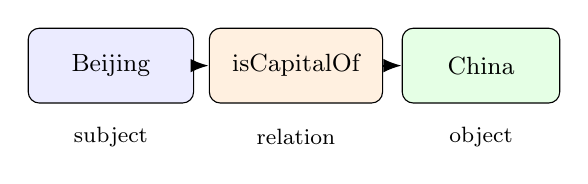
\begin{tikzpicture}[>=Latex, every node/.style={font=\small}]
      \node[draw, rounded corners, fill=blue!8, minimum width=2.1cm, minimum height=0.95cm] (s) at (0,0) {Beijing};
      \node[draw, rounded corners, fill=orange!12, minimum width=2.2cm, minimum height=0.95cm] (p) at (2.35,0) {isCapitalOf};
      \node[draw, rounded corners, fill=green!10, minimum width=2.0cm, minimum height=0.95cm] (o) at (4.7,0) {China};
      \draw[->, thick] (s) -- (p);
      \draw[->, thick] (p) -- (o);
      \node[font=\footnotesize] at (0,-0.9) {subject};
      \node[font=\footnotesize] at (2.35,-0.9) {relation};
      \node[font=\footnotesize] at (4.7,-0.9) {object};
    \end{tikzpicture}
    \end{center}
  \end{column}
\end{columns}
\plainidea{Representation breaks one sentence into clear parts so the machine can store the fact and connect it later.}
\end{frame}

% 9
\setslideref{AIMA4e Ch.10 pp.314--343; Poole3e Ch.16 pp.701--730}
\begin{frame}{Reasoning Needs Explicit Facts}
\keyquestion{How can a machine go from known facts to a new conclusion?}
\begin{center}
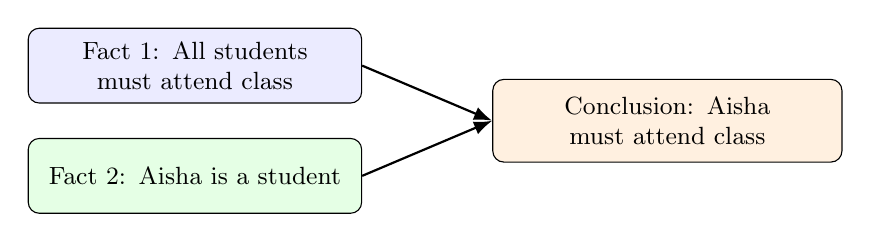
\begin{tikzpicture}[>=Latex, every node/.style={font=\small}]
  \node[draw, rounded corners, fill=blue!8, text width=4.0cm, align=center, minimum height=0.95cm] (f1) at (0,1.0) {Fact 1: All students must attend class};
  \node[draw, rounded corners, fill=green!10, text width=4.0cm, align=center, minimum height=0.95cm] (f2) at (0,-0.4) {Fact 2: Aisha is a student};
  \node[draw, rounded corners, fill=orange!12, text width=4.2cm, align=center, minimum height=1.05cm] (c) at (6.0,0.3) {Conclusion: Aisha must attend class};
  \draw[->, thick] (f1.east) -- (c.west);
  \draw[->, thick] (f2.east) -- (c.west);
\end{tikzpicture}
\end{center}
\plainidea{If the system stores facts and rules explicitly, it can combine them step by step to derive a new answer.}
\end{frame}

% 10
\setslideref{AIMA4e Ch.10 pp.314--343; Poole3e Ch.16 pp.701--730}
\begin{frame}{Symbols Connect Perception to Action}
\keyquestion{Why do symbols matter when an AI system must act in the world?}
\begin{center}
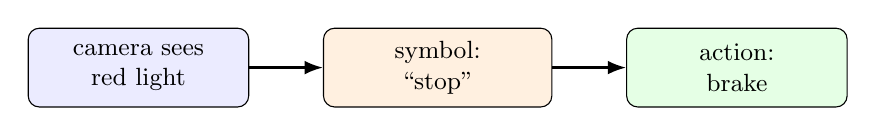
\begin{tikzpicture}[>=Latex, every node/.style={font=\small}]
  \node[draw, rounded corners, fill=blue!8, minimum width=2.8cm, minimum height=1.0cm, align=center] (see) at (0,0) {camera sees\\red light};
  \node[draw, rounded corners, fill=orange!12, minimum width=2.9cm, minimum height=1.0cm, align=center] (symbol) at (3.8,0) {symbol: \\ ``stop''};
  \node[draw, rounded corners, fill=green!10, minimum width=2.8cm, minimum height=1.0cm, align=center] (act) at (7.6,0) {action:\\ brake};
  \draw[->, thick] (see) -- (symbol);
  \draw[->, thick] (symbol) -- (act);
\end{tikzpicture}
\end{center}
\begin{itemize}
  \item Sensors produce raw data.
  \item Representation maps that raw data to a meaningful symbol.
  \item The symbol helps the agent choose the correct action.
\end{itemize}
\plainidea{Representation is the bridge between perception and decision.}
\end{frame}

% 11
\setslideref{AIMA4e Ch.10 pp.314--343; Poole3e Ch.16 pp.701--730}
\begin{frame}{Types of Knowledge an Agent Needs}
\keyquestion{Does one useful agent need only factual knowledge?}
\small
\begin{tabular}{@{}p{0.2\linewidth}p{0.72\linewidth}@{}}
\toprule
\textbf{Type} & \textbf{Simple meaning and example} \\
\midrule
Declarative & facts about the world. Example: ``Beijing is in China.'' \\
Procedural & how to do something. Example: how to book a ticket \\
Semantic & concepts and relations. Example: student -- enrolledIn -- module \\
Episodic & memory of past events. Example: the last support ticket \\
Meta-knowledge & what is known, missing, or uncertain. Example: ``I need more evidence.'' \\
\bottomrule
\end{tabular}
\plainidea{Real agents mix facts, procedures, concepts, memories, and uncertainty about what they know.}
\end{frame}

% 12
\setslideref{AIMA4e Ch.10 pp.314--343; Poole3e Ch.16 pp.701--730}
\begin{frame}{Core Terms for Today}
\keyquestion{What six words should you keep in mind during this lecture?}
\begin{center}
\begin{tabular}{@{}ll@{}}
\toprule
Term & Meaning \\
\midrule
Knowledge representation & A formal way to store meaning \\
Entity & A thing, person, place, or object \\
Relation & A named link between two entities \\
Attribute & A property of one entity \\
Triple & Subject -- predicate -- object fact \\
Identifier & A unique label for one entity \\
\bottomrule
\end{tabular}
\end{center}
\plainidea{If you understand these six terms, the rest of the lecture becomes much easier to follow.}
\end{frame}

% 13
\setslideref{AIMA4e Ch.10 pp.314--343; Poole3e Ch.16 pp.701--730}
\begin{frame}{Personal Assistant Example}
\keyquestion{What must an assistant understand in a query like ``Play a song by Da Zhang Wei''?}
\begin{columns}[T,onlytextwidth]
  \begin{column}{0.42\textwidth}
    \begin{tcolorbox}[colback=questionbg,colframe=questionframe,boxrule=0.7pt,title=User query]
    ``Play a song by Da Zhang Wei''
    \end{tcolorbox}
  \end{column}
  \begin{column}{0.54\textwidth}
    \begin{itemize}
      \item detect the entity: Da Zhang Wei
      \item detect the intent: play music
      \item retrieve the linked facts: artist, songs, platform, permissions
    \end{itemize}
  \end{column}
\end{columns}
\plainidea{The assistant must identify what the user means, not only what words the user typed.}
\end{frame}

% 14
\setslideref{AIMA4e Ch.10 pp.314--343; Poole3e Ch.16 pp.701--730}
\begin{frame}{Assistant Understanding Pipeline}
\keyquestion{What steps happen between the user's question and the system's answer?}
\begin{center}
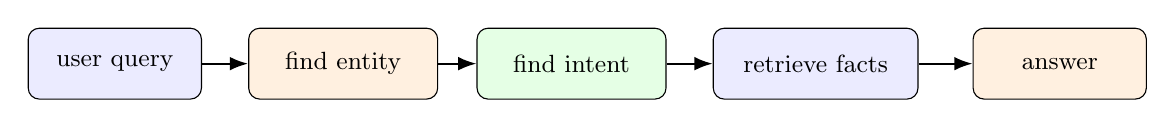
\begin{tikzpicture}[>=Latex, every node/.style={font=\small}]
  \node[draw, rounded corners, fill=blue!8, minimum width=2.2cm, minimum height=0.9cm, align=center] (q) at (0,0) {user query};
  \node[draw, rounded corners, fill=orange!12, minimum width=2.4cm, minimum height=0.9cm, align=center] (e) at (2.9,0) {find entity};
  \node[draw, rounded corners, fill=green!10, minimum width=2.4cm, minimum height=0.9cm, align=center] (i) at (5.8,0) {find intent};
  \node[draw, rounded corners, fill=blue!8, minimum width=2.6cm, minimum height=0.9cm, align=center] (r) at (8.9,0) {retrieve facts};
  \node[draw, rounded corners, fill=orange!12, minimum width=2.2cm, minimum height=0.9cm, align=center] (a) at (12.0,0) {answer};
  \draw[->, thick] (q) -- (e);
  \draw[->, thick] (e) -- (i);
  \draw[->, thick] (i) -- (r);
  \draw[->, thick] (r) -- (a);
\end{tikzpicture}
\end{center}
\plainidea{A good answer is usually the result of several small steps, not one magic jump from text to text.}
\end{frame}

% 15
\setslideref{AIMA4e Ch.10 pp.314--343; Poole3e Ch.16 pp.701--730; https://developers.google.com/search/docs}
\begin{frame}{Why Search Uses Connected Facts}
\keyquestion{Why do search systems connect facts instead of storing isolated lines of text?}
\begin{center}
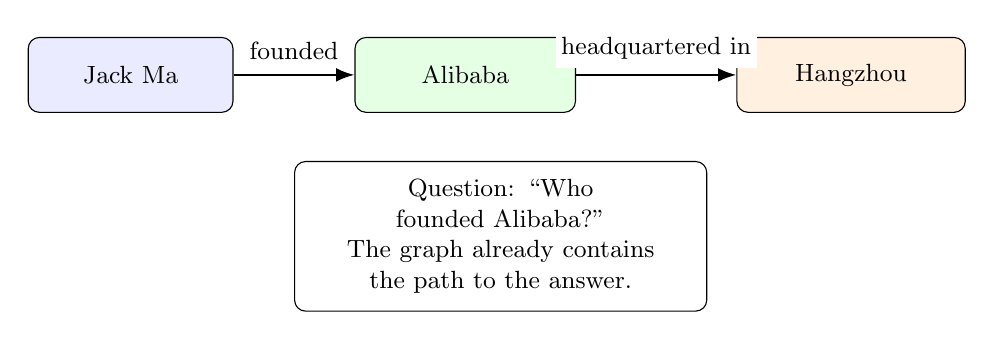
\begin{tikzpicture}[>=Latex, every node/.style={font=\small}]
  \node[draw, rounded corners, fill=blue!8, minimum width=2.6cm, minimum height=0.95cm] (jack) at (0,0.2) {Jack Ma};
  \node[draw, rounded corners, fill=green!10, minimum width=2.8cm, minimum height=0.95cm] (ali) at (4.25,0.2) {Alibaba};
  \node[draw, rounded corners, fill=orange!12, minimum width=2.9cm, minimum height=0.95cm] (hang) at (9.15,0.2) {Hangzhou};
  \draw[->, thick] (jack) -- node[midway, above=2pt, fill=white, inner xsep=2pt]{founded} (ali);
  \draw[->, thick] (ali) -- node[midway, above=2pt, fill=white, inner xsep=2pt]{headquartered in} (hang);
  \node[draw, rounded corners, fill=white, text width=5.0cm, minimum height=1.9cm, align=center] at (4.7,-1.85) {Question: ``Who founded Alibaba?''\\The graph already contains the path to the answer.};
\end{tikzpicture}
\end{center}
\plainidea{Connected facts let the system move from one entity to another instead of scanning unrelated text every time.}
\end{frame}

% 16
\setslideref{AIMA4e Ch.10 pp.314--343; Poole3e Ch.16 pp.701--730; https://developers.google.com/search/docs}
\begin{frame}{Example: Knowledge Panel in Search}
\keyquestion{What does structured knowledge look like in a real search result?}
\begin{center}
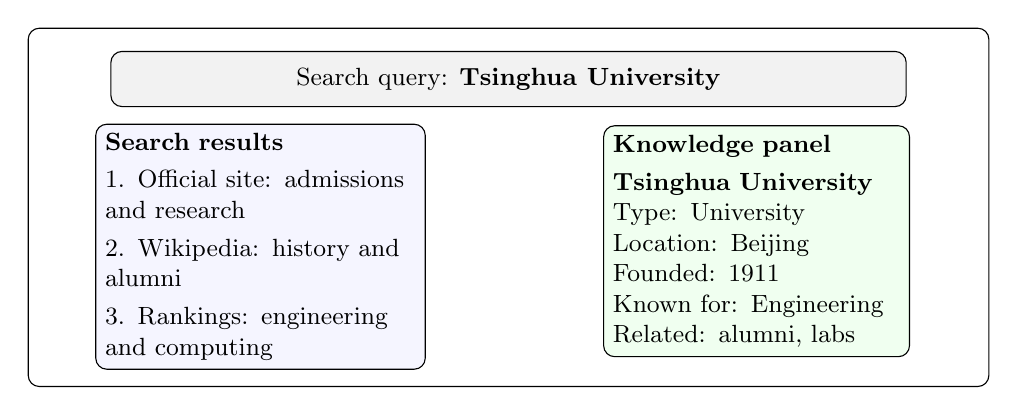
\begin{tikzpicture}[every node/.style={font=\small}]
  \node[draw, rounded corners, minimum width=12.2cm, minimum height=4.55cm, fill=white] (browser) at (0,0.15) {};
  \node[draw, rounded corners, fill=gray!10, minimum width=10.1cm, minimum height=0.7cm, align=center] at (0,1.78) {Search query: \textbf{Tsinghua University}};

  \node[draw, rounded corners, fill=blue!4, text width=3.95cm, minimum height=2.75cm, align=left] at (-3.15,-0.35) {\textbf{Search results}\\[0.25em]
  1. Official site: admissions and research\\[0.3em]
  2. Wikipedia: history and alumni\\[0.3em]
  3. Rankings: engineering and computing};

  \node[draw, rounded corners, fill=green!6, text width=3.65cm, minimum height=2.75cm, align=left] at (3.15,-0.28) {\textbf{Knowledge panel}\\[0.3em]\textbf{Tsinghua University}\\Type: University\\Location: Beijing\\Founded: 1911\\Known for: Engineering\\Related: alumni, labs};
\end{tikzpicture}
\end{center}
\plainidea{A knowledge panel is a user-facing view of structured facts.}
\end{frame}

% 17
\setslideref{AIMA4e Ch.10 pp.314--343; Poole3e Ch.16 pp.701--730}
\begin{frame}{Topic Pages Use the Same Idea}
\keyquestion{What changes when a platform links topics, questions, and people?}
\begin{center}
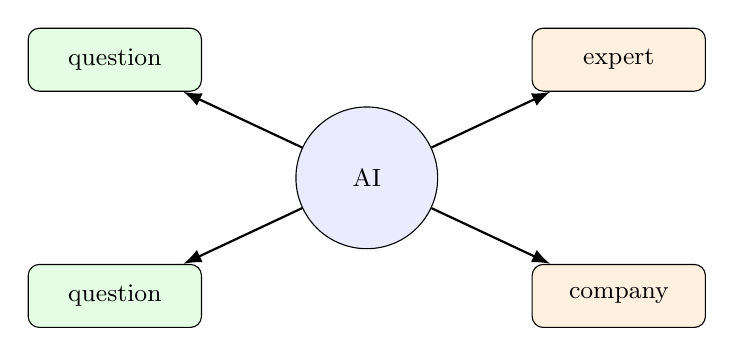
\begin{tikzpicture}[>=Latex, every node/.style={font=\small}]
  \node[draw, circle, fill=blue!8, minimum size=1.8cm] (topic) at (0,0) {AI};
  \node[draw, rounded corners, fill=green!10, minimum width=2.2cm, minimum height=0.8cm] (q1) at (-3.2,1.5) {question};
  \node[draw, rounded corners, fill=green!10, minimum width=2.2cm, minimum height=0.8cm] (q2) at (-3.2,-1.5) {question};
  \node[draw, rounded corners, fill=orange!12, minimum width=2.2cm, minimum height=0.8cm] (p1) at (3.2,1.5) {expert};
  \node[draw, rounded corners, fill=orange!12, minimum width=2.2cm, minimum height=0.8cm] (p2) at (3.2,-1.5) {company};
  \draw[->, thick] (topic) -- (q1);
  \draw[->, thick] (topic) -- (q2);
  \draw[->, thick] (topic) -- (p1);
  \draw[->, thick] (topic) -- (p2);
\end{tikzpicture}
\end{center}
\plainidea{Once items are linked by meaning, the system can organise a topic page instead of showing random isolated content.}
\end{frame}

% 18
\setslideref{AIMA4e Ch.10 pp.314--343; Poole3e Ch.16 pp.701--730}
\begin{frame}{Where Do We See Knowledge Representation Already?}
\keyquestion{In which everyday AI systems do we already see the same representation idea?}
\begin{columns}[T,onlytextwidth]
  \begin{column}{0.32\textwidth}
    \begin{tcolorbox}[colback=questionbg,colframe=questionframe,boxrule=0.7pt,title=Assistant]
    Maps query to\\entity + intent + facts
    \end{tcolorbox}
  \end{column}
  \begin{column}{0.32\textwidth}
    \begin{tcolorbox}[colback=plainbg,colframe=plainframe,boxrule=0.7pt,title=Search]
    Uses linked facts\\for panels and direct answers
    \end{tcolorbox}
  \end{column}
  \begin{column}{0.32\textwidth}
    \begin{tcolorbox}[colback=notationbg,colframe=notationframe,boxrule=0.7pt,title=Enterprise agent]
    Connects documents, people, systems, and policies
    \end{tcolorbox}
  \end{column}
\end{columns}
\plainidea{The products look different, but the underlying idea is the same: store meaning in a structure the system can follow.}
\end{frame}

% 19
\setslideref{AIMA4e Ch.10 pp.314--343; Poole3e Ch.16 pp.701--730}
\begin{frame}{Triple Representation}
\keyquestion{What is the smallest useful fact unit in many graph systems?}
\[
(\text{subject},\ \text{predicate},\ \text{object})
\]
\begin{center}
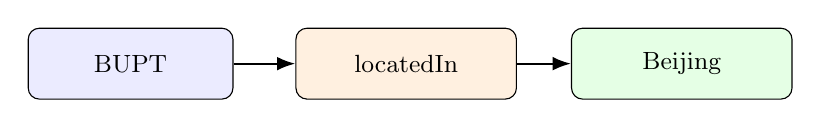
\begin{tikzpicture}[>=Latex, every node/.style={font=\small}]
  \node[draw, rounded corners, fill=blue!8, minimum width=2.6cm, minimum height=0.9cm] (s) at (0,0) {BUPT};
  \node[draw, rounded corners, fill=orange!12, minimum width=2.8cm, minimum height=0.9cm] (p) at (3.5,0) {locatedIn};
  \node[draw, rounded corners, fill=green!10, minimum width=2.8cm, minimum height=0.9cm] (o) at (7.0,0) {Beijing};
  \draw[->, thick] (s) -- (p);
  \draw[->, thick] (p) -- (o);
\end{tikzpicture}
\end{center}
\notationblock{subject: the thing we are talking about\\
predicate: the named relation\\
object: the thing or value linked by that relation}
\plainidea{A triple is small, simple, and reusable. Many large knowledge graphs are built from many triples.}
\end{frame}

% 20
\setslideref{AIMA4e Ch.10 pp.314--343; Poole3e Ch.16 pp.701--730}
\begin{frame}{Entities, Relations, and Attributes}
\keyquestion{How do we tell apart a thing, a link, and a property?}
\begin{columns}[T,onlytextwidth]
  \begin{column}{0.31\textwidth}
    \begin{tcolorbox}[colback=questionbg,colframe=questionframe,boxrule=0.7pt,title=Entity]
    A thing in the world\\
    Example: ``Aisha''\\``QMUL''\\``Module EBU6505''
    \end{tcolorbox}
  \end{column}
  \begin{column}{0.31\textwidth}
    \begin{tcolorbox}[colback=plainbg,colframe=plainframe,boxrule=0.7pt,title=Relation]
    A link between entities\\
    Example: enrolledIn\\teaches\\locatedIn
    \end{tcolorbox}
  \end{column}
  \begin{column}{0.31\textwidth}
    \begin{tcolorbox}[colback=notationbg,colframe=notationframe,boxrule=0.7pt,title=Attribute]
    A property of one entity\\
    Example: birthDate\\moduleCode\\roomNumber
    \end{tcolorbox}
  \end{column}
\end{columns}
\plainidea{Do not mix them up: entity = thing, relation = link, attribute = property.}
\end{frame}

% 21
\setslideref{AIMA4e Ch.10 pp.314--343; Poole3e Ch.16 pp.701--730}
\begin{frame}{Why Identifiers Matter}
\keyquestion{Why is a unique identifier better than only a name string?}
\begin{tcolorbox}[colback=questionbg,colframe=questionframe,boxrule=0.7pt,title=Problem]
Two different people can both be called ``Ali''. The name is helpful for humans, but it is not enough for the machine.
\end{tcolorbox}
\vspace{0.4em}
\begin{center}
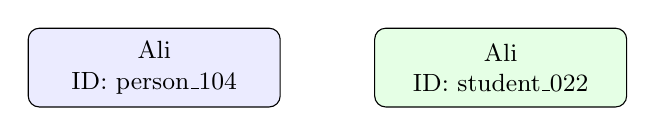
\begin{tikzpicture}[every node/.style={font=\small}]
  \node[draw, rounded corners, fill=blue!8, minimum width=3.2cm, minimum height=1.0cm, align=center] at (-2.2,0) {Ali\\ID: person\_104};
  \node[draw, rounded corners, fill=green!10, minimum width=3.2cm, minimum height=1.0cm, align=center] at (2.2,0) {Ali\\ID: student\_022};
\end{tikzpicture}
\end{center}
\begin{itemize}
  \item names are human-friendly
  \item identifiers keep different entities separate
\end{itemize}
\plainidea{Names help users. Identifiers help the machine keep different entities separate.}
\end{frame}

% 22
\setslideref{AIMA4e Ch.10 pp.314--343; Poole3e Ch.16 pp.701--730}
\begin{frame}{Schema Graph Versus Instance Graph}
\keyquestion{What is the difference between the pattern of a graph and the actual facts inside it?}
\begin{columns}[T,onlytextwidth]
  \begin{column}{0.48\textwidth}
    \begin{tcolorbox}[colback=questionbg,colframe=questionframe,boxrule=0.7pt,title=Schema graph]
    Defines the allowed kinds of nodes and links.
    \end{tcolorbox}
  \end{column}
  \begin{column}{0.48\textwidth}
    \begin{tcolorbox}[colback=plainbg,colframe=plainframe,boxrule=0.7pt,title=Instance graph]
    Stores one real fact that follows that pattern.
    \end{tcolorbox}
  \end{column}
\end{columns}
\vspace{-0.1em}
\begin{center}
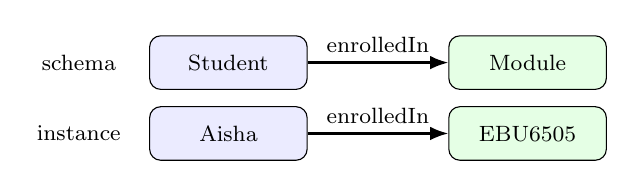
\begin{tikzpicture}[>=Latex, every node/.style={font=\footnotesize}]
  \node[draw, rounded corners, fill=blue!8, minimum width=2.0cm, minimum height=0.68cm] (st) at (0,0.42) {Student};
  \node[draw, rounded corners, fill=green!10, minimum width=2.0cm, minimum height=0.68cm] (mod) at (3.8,0.42) {Module};
  \draw[->, thick] (st) -- node[above]{enrolledIn} (mod);
  \node[draw, rounded corners, fill=blue!8, minimum width=2.0cm, minimum height=0.68cm] (a) at (0,-0.48) {Aisha};
  \node[draw, rounded corners, fill=green!10, minimum width=2.0cm, minimum height=0.68cm] (m) at (3.8,-0.48) {EBU6505};
  \draw[->, thick] (a) -- node[above]{enrolledIn} (m);
  \node[font=\footnotesize] at (-1.9,0.42) {schema};
  \node[font=\footnotesize] at (-1.9,-0.48) {instance};
\end{tikzpicture}
\end{center}
\plainidea{Schema gives the pattern. Instance data fills that pattern with real facts.}
\end{frame}

% 23
\setslideref{AIMA4e Ch.10 pp.314--343; Poole3e Ch.16 pp.701--730}
\begin{frame}{From Knowledge Representation to Agent Memory}
\keyquestion{Why do modern agents need structured memory instead of only prompt text?}
\begin{columns}[T,onlytextwidth]
  \begin{column}{0.48\textwidth}
    \begin{tcolorbox}[colback=questionbg,colframe=questionframe,boxrule=0.7pt,title=Prompt-only memory]
    Long, noisy, expensive to search\\
    Easy to forget exact facts
    \end{tcolorbox}
  \end{column}
  \begin{column}{0.48\textwidth}
    \begin{tcolorbox}[colback=plainbg,colframe=plainframe,boxrule=0.7pt,title=Structured memory]
    Facts are normalized and linked\\
    Easier to retrieve exact evidence
    \end{tcolorbox}
  \end{column}
\end{columns}
\plainidea{A long prompt is temporary context. A structured memory is reusable knowledge.}
\end{frame}

% 24
\setslideref{AIMA4e Ch.10 pp.314--343; Poole3e Ch.16 pp.701--730}
\begin{frame}{Memory Layers in Modern Agents}
\keyquestion{What kinds of memory should a useful agent keep?}
\begin{center}
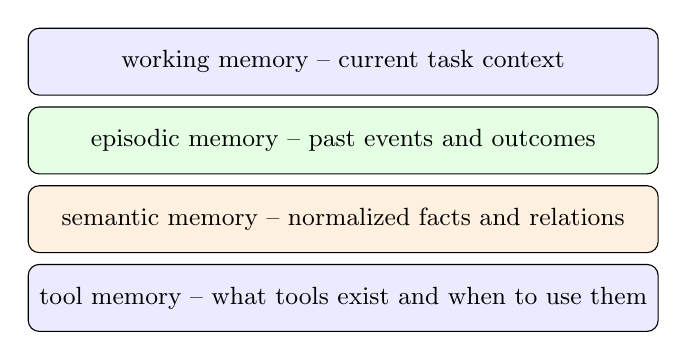
\begin{tikzpicture}[every node/.style={font=\small}]
  \node[draw, rounded corners, fill=blue!8, minimum width=8.0cm, minimum height=0.85cm] at (0,1.8) {working memory -- current task context};
  \node[draw, rounded corners, fill=green!10, minimum width=8.0cm, minimum height=0.85cm] at (0,0.8) {episodic memory -- past events and outcomes};
  \node[draw, rounded corners, fill=orange!12, minimum width=8.0cm, minimum height=0.85cm] at (0,-0.2) {semantic memory -- normalized facts and relations};
  \node[draw, rounded corners, fill=blue!8, minimum width=8.0cm, minimum height=0.85cm] at (0,-1.2) {tool memory -- what tools exist and when to use them};
\end{tikzpicture}
\end{center}
\plainidea{Not all memory is the same. Some memory is short-term, while some memory must survive across many tasks.}
\end{frame}

% 25
\setslideref{AIMA4e Ch.10 pp.314--343; Poole3e Ch.16 pp.701--730}
\begin{frame}{Why Structured Memory Beats Raw Logs}
\keyquestion{Why is a graph or table often better than a long chat log?}
\begin{columns}[T,onlytextwidth]
  \begin{column}{0.48\textwidth}
    \begin{tcolorbox}[colback=questionbg,colframe=questionframe,boxrule=0.7pt,title=Raw log]
    Repeated wording\\
    Missing exact links\\
    Hard to audit
    \end{tcolorbox}
  \end{column}
  \begin{column}{0.48\textwidth}
    \begin{tcolorbox}[colback=plainbg,colframe=plainframe,boxrule=0.7pt,title=Structured memory]
    Explicit entities and links\\
    Easier retrieval\\
    Clearer provenance
    \end{tcolorbox}
  \end{column}
\end{columns}
\plainidea{Structured memory reduces ambiguity and makes later reasoning easier to inspect.}
\end{frame}

% 26
\setslideref{AIMA4e Ch.10 pp.314--343; Poole3e Ch.16 pp.701--730}
\begin{frame}{Agent Memory Update Loop}
\keyquestion{How does an agent turn new evidence into usable memory?}
\begin{center}
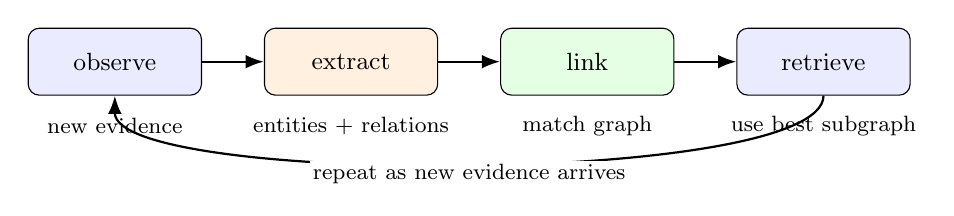
\begin{tikzpicture}[>=Latex, every node/.style={font=\small}]
  \node[draw, rounded corners, fill=blue!8, minimum width=2.2cm, minimum height=0.85cm] (o) at (0,0.1) {observe};
  \node[draw, rounded corners, fill=orange!12, minimum width=2.2cm, minimum height=0.85cm] (x) at (3.0,0.1) {extract};
  \node[draw, rounded corners, fill=green!10, minimum width=2.2cm, minimum height=0.85cm] (l) at (6.0,0.1) {link};
  \node[draw, rounded corners, fill=blue!8, minimum width=2.2cm, minimum height=0.85cm] (r) at (9.0,0.1) {retrieve};
  \draw[->, thick] (o) -- (x);
  \draw[->, thick] (x) -- (l);
  \draw[->, thick] (l) -- (r);
  \node[font=\footnotesize] at (0,-0.72) {new evidence};
  \node[font=\footnotesize] at (3.0,-0.72) {entities + relations};
  \node[font=\footnotesize] at (6.0,-0.72) {match graph};
  \node[font=\footnotesize] at (9.0,-0.72) {use best subgraph};
  \draw[->, thick] (r.south) .. controls +(down:1.15cm) and +(down:1.15cm) .. (o.south);
  \node[font=\footnotesize, fill=white, inner sep=1pt] at (4.5,-1.32) {repeat as new evidence arrives};
\end{tikzpicture}
\end{center}
\plainidea{Useful memory is not static. The agent keeps updating the graph as it learns new evidence.}
\end{frame}

% 27
\setslideref{AIMA4e Ch.10 pp.314--343; Poole3e Ch.16 pp.701--730; https://developers.google.com/search/docs}
\begin{frame}{Case Study: Search Engines Reason Over KGs}
\keyquestion{How can a search engine use a graph to answer faster and more clearly?}
\begin{columns}[T,onlytextwidth]
  \begin{column}{0.52\textwidth}
    \begin{itemize}
      \item map the query to entities
      \item follow useful relation paths
      \item rank candidate answers
      \item show a short answer or panel
    \end{itemize}
  \end{column}
  \begin{column}{0.44\textwidth}
    \begin{center}
    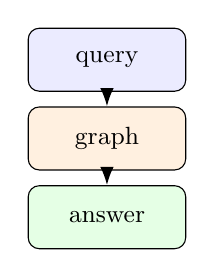
\begin{tikzpicture}[>=Latex, every node/.style={font=\small}]
      \node[draw, rounded corners, fill=blue!8, minimum width=2.0cm, minimum height=0.8cm] (q) at (0,0.8) {query};
      \node[draw, rounded corners, fill=orange!12, minimum width=2.0cm, minimum height=0.8cm] (g) at (0,-0.2) {graph};
      \node[draw, rounded corners, fill=green!10, minimum width=2.0cm, minimum height=0.8cm] (a) at (0,-1.2) {answer};
      \draw[->, thick] (q) -- (g);
      \draw[->, thick] (g) -- (a);
    \end{tikzpicture}
    \end{center}
  \end{column}
\end{columns}
\plainidea{The graph helps the system move quickly from a query to a supported answer path.}
\end{frame}

% 28
\setslideref{AIMA4e Ch.10 pp.314--343; Poole3e Ch.16 pp.701--730; https://developers.google.com/search/docs}
\begin{frame}{Search Example Workflow}
\keyquestion{How might a graph help with ``best EV charging options near campus''?}
\begin{center}
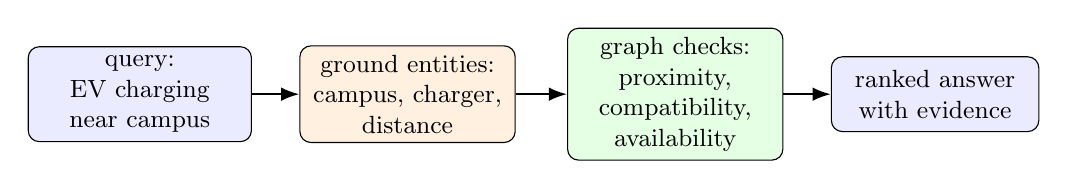
\begin{tikzpicture}[>=Latex, every node/.style={font=\small}]
  \node[draw, rounded corners, fill=blue!8, text width=2.6cm, minimum height=0.95cm, align=center] (q) at (0,0) {query:\\ EV charging near campus};
  \node[draw, rounded corners, fill=orange!12, text width=2.5cm, minimum height=0.95cm, align=center] (e) at (3.4,0) {ground entities:\\ campus, charger, distance};
  \node[draw, rounded corners, fill=green!10, text width=2.5cm, minimum height=0.95cm, align=center] (g) at (6.8,0) {graph checks:\\ proximity, compatibility, availability};
  \node[draw, rounded corners, fill=blue!8, text width=2.4cm, minimum height=0.95cm, align=center] (a) at (10.1,0) {ranked answer\\ with evidence};
  \draw[->, thick] (q) -- (e);
  \draw[->, thick] (e) -- (g);
  \draw[->, thick] (g) -- (a);
\end{tikzpicture}
\end{center}
\plainidea{The graph lets the search system combine several conditions instead of matching only keywords.}
\end{frame}

% 29
\setslideref{AIMA4e Ch.10 pp.314--343; Poole3e Ch.16 pp.701--730; https://developers.google.com/search/docs}
\begin{frame}{Search Engine KG Failure Modes}
\keyquestion{What can go wrong if the stored knowledge is weak or outdated?}
\begin{columns}[T,onlytextwidth]
  \begin{column}{0.48\textwidth}
    \begin{tcolorbox}[colback=questionbg,colframe=questionframe,boxrule=0.7pt,title=Common failures]
    stale facts\\
    poor entity linking\\
    missing facts\\
    missing provenance
    \end{tcolorbox}
  \end{column}
  \begin{column}{0.48\textwidth}
    \begin{tcolorbox}[colback=plainbg,colframe=plainframe,boxrule=0.7pt,title=Common fixes]
    freshness checks\\
    confidence thresholds\\
    source traces\\
    human review for risky cases
    \end{tcolorbox}
  \end{column}
\end{columns}
\plainidea{A knowledge graph is useful only if the links are accurate, current, and traceable.}
\end{frame}

% 30
\setslideref{AIMA4e Ch.10 pp.314--343; Poole3e Ch.16 pp.701--730}
\begin{frame}{Agents Reasoning Over Internal Company Knowledge}
\keyquestion{Why do companies want agents to reason over internal knowledge?}
\begin{itemize}
  \item useful facts are spread across documents, tickets, systems, and people
  \item the agent must connect services, owners, changes, and policies
  \item this helps answer questions like ``who owns service X?'' or ``what changed last week?''
\end{itemize}
\plainidea{Enterprise knowledge is not one document. It is a network of connected facts spread across many systems.}
\end{frame}

% 31
\setslideref{AIMA4e Ch.10 pp.314--343; Poole3e Ch.16 pp.701--730}
\begin{frame}{Enterprise Reasoning Example}
\keyquestion{What might an internal support agent do during an incident?}
\begin{center}
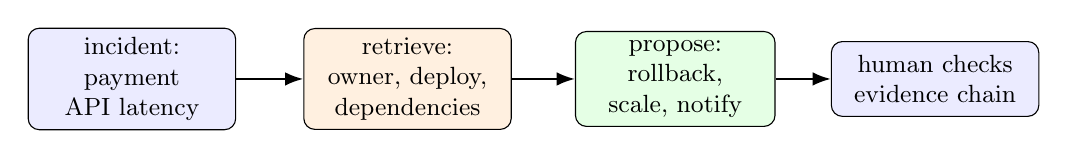
\begin{tikzpicture}[>=Latex, every node/.style={font=\small}]
  \node[draw, rounded corners, fill=blue!8, text width=2.4cm, minimum height=0.95cm, align=center] (i) at (0,0) {incident:\\ payment API latency};
  \node[draw, rounded corners, fill=orange!12, text width=2.4cm, minimum height=0.95cm, align=center] (r) at (3.5,0) {retrieve:\\ owner, deploy, dependencies};
  \node[draw, rounded corners, fill=green!10, text width=2.3cm, minimum height=0.95cm, align=center] (p) at (6.9,0) {propose:\\ rollback, scale, notify};
  \node[draw, rounded corners, fill=blue!8, text width=2.4cm, minimum height=0.95cm, align=center] (h) at (10.2,0) {human checks\\ evidence chain};
  \draw[->, thick] (i) -- (r);
  \draw[->, thick] (r) -- (p);
  \draw[->, thick] (p) -- (h);
\end{tikzpicture}
\end{center}
\plainidea{The agent does not act blindly. It gathers linked evidence first, then proposes a grounded next step.}
\end{frame}

% 32
\setslideref{AIMA4e Ch.10 pp.314--343; Poole3e Ch.16 pp.701--730}
\begin{frame}{Governance for Internal Knowledge Agents}
\keyquestion{Why can an internal knowledge agent not be given unlimited freedom?}
\begin{columns}[T,onlytextwidth]
  \begin{column}{0.48\textwidth}
    \begin{itemize}
      \item role-based access control
      \item provenance for each retrieved fact
    \end{itemize}
  \end{column}
  \begin{column}{0.48\textwidth}
    \begin{itemize}
      \item privacy and security filters
      \item human review for high-risk actions
    \end{itemize}
  \end{column}
\end{columns}
\plainidea{Internal knowledge is powerful, so the agent must be accurate, traceable, and controlled.}
\end{frame}

% 33
\setslideref{AIMA4e Ch.10 pp.314--343; Poole3e Ch.16 pp.701--730; https://modelcontextprotocol.io/specification/; https://openai.github.io/openai-agents-python/}
\begin{frame}{Modern AI Assistants Reason About Tool Choice}
\keyquestion{Before calling a tool, what does an assistant need to decide?}
\begin{itemize}
  \item do I need a factual lookup?
  \item do I need to perform an action?
  \item am I uncertain enough that I should ask a clarifying question first?
\end{itemize}
\plainidea{Good agents do not call tools randomly. They first decide what kind of job they are trying to do.}
\end{frame}

% 34
\setslideref{AIMA4e Ch.10 pp.314--343; Poole3e Ch.16 pp.701--730; https://modelcontextprotocol.io/specification/; https://openai.github.io/openai-agents-python/}
\begin{frame}{Tool Selection Policy Pattern}
\keyquestion{What simple policy can an agent follow when choosing a tool?}
\begin{center}
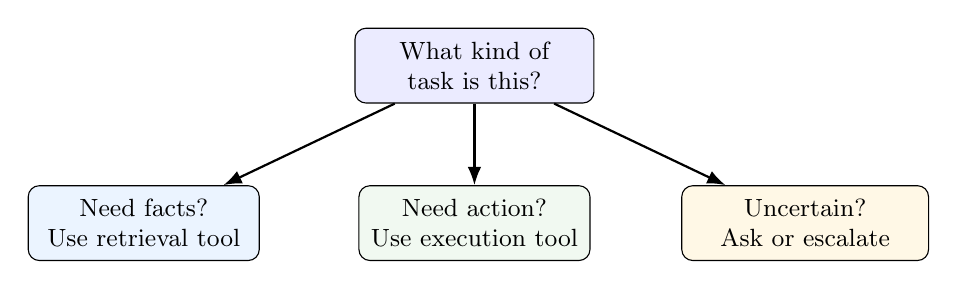
\begin{tikzpicture}[>=Latex, every node/.style={font=\small}]
  \node[draw, rounded corners, fill=blue!8, text width=2.8cm, minimum height=0.95cm, align=center] (task) at (0,0) {What kind of task is this?};
  \node[draw, rounded corners, fill=questionbg, text width=2.7cm, minimum height=0.95cm, align=center] (fact) at (-4.2,-2.0) {Need facts?\\Use retrieval tool};
  \node[draw, rounded corners, fill=plainbg, text width=2.7cm, minimum height=0.95cm, align=center] (act) at (0,-2.0) {Need action?\\Use execution tool};
  \node[draw, rounded corners, fill=notationbg, text width=2.9cm, minimum height=0.95cm, align=center] (ask) at (4.2,-2.0) {Uncertain?\\Ask or escalate};
  \draw[->, thick] (task) -- (fact);
  \draw[->, thick] (task) -- (act);
  \draw[->, thick] (task) -- (ask);
\end{tikzpicture}
\end{center}
\plainidea{A simple decision policy already prevents many bad tool calls.}
\end{frame}

% 35
\setslideref{AIMA4e Ch.10 pp.314--343; Poole3e Ch.16 pp.701--730; https://modelcontextprotocol.io/specification/; https://openai.github.io/openai-agents-python/}
\begin{frame}{Why Separate Planning From Execution?}
\keyquestion{Why do many agent systems keep planning and execution separate?}
\begin{center}
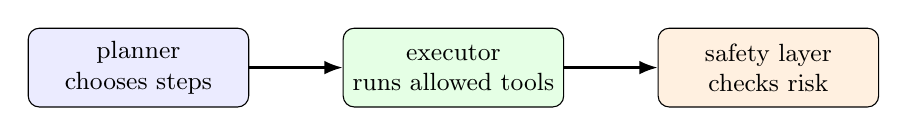
\begin{tikzpicture}[>=Latex, every node/.style={font=\small}]
  \node[draw, rounded corners, fill=blue!8, minimum width=2.8cm, minimum height=1.0cm, align=center] (planner) at (0,0) {planner\\chooses steps};
  \node[draw, rounded corners, fill=green!10, minimum width=2.8cm, minimum height=1.0cm, align=center] (executor) at (4.0,0) {executor\\runs allowed tools};
  \node[draw, rounded corners, fill=orange!12, minimum width=2.8cm, minimum height=1.0cm, align=center] (safety) at (8.0,0) {safety layer\\checks risk};
  \draw[->, thick] (planner) -- (executor);
  \draw[->, thick] (executor) -- (safety);
\end{tikzpicture}
\end{center}
\plainidea{This separation makes the system easier to control, debug, and audit.}
\end{frame}

% 36
\setslideref{AIMA4e Ch.10 pp.314--343; Poole3e Ch.16 pp.701--730}
\begin{frame}{In-Class Exercises}
\exercisebreakcontent{Keep the graph small. A clear tiny graph is better than a large messy one.}
\end{frame}

% 37
\setslideref{AIMA4e Ch.10 pp.314--343; Poole3e Ch.16 pp.701--730}
\begin{frame}{Key Takeaways}
\keyquestion{What should you remember most from today's lecture?}
\begin{itemize}
  \item AI systems need explicit knowledge structures, not only natural language.
  \item Triples are a simple and powerful way to store facts.
  \item Entities, relations, attributes, and identifiers must be distinguished clearly.
  \item Search systems and modern agents both benefit from structured knowledge.
\end{itemize}
\plainidea{If a machine can store facts clearly, it can retrieve better and reason better.}
\end{frame}

% 38
\setslideref{AIMA4e Ch.10 pp.314--343; Poole3e Ch.16 pp.701--730}
\begin{frame}{Further Study}
\begin{itemize}
  \item Read Poole Chapter 16 and AIMA Chapter 10.
  \item Practice: Poole Ch.16, Exercises 16.2, 16.3, 16.5, 16.6, and 16.9.
  \item AIMA knowledge-representation exercise page: 2, 9, 13, 16, and 26.
  \item Try writing 5 triples for one domain you know well.
  \item Ask yourself: which facts are entities, which are attributes, and which are relations?
  \item Prepare for Day 3: we move from simple representation to stronger graph foundations.
\end{itemize}
\end{frame}

\end{document}
